\documentclass[border=6pt]{standalone}
\usepackage[T1]{fontenc}
\usepackage{lmodern}
\usepackage{tikz}
\begin{document}
\hyphenpenalty=10000 \exhyphenpenalty=10000
% Gap between reported confidence and observed accuracy, by confidence group.
% Values are the reported group table (Hoang, Figure 11): 0.01 0.17 0.27 0.16 0.07 0.03.
% Scale: 1.0 of gap = 20 cm, so 0.27 = 5.4 cm.
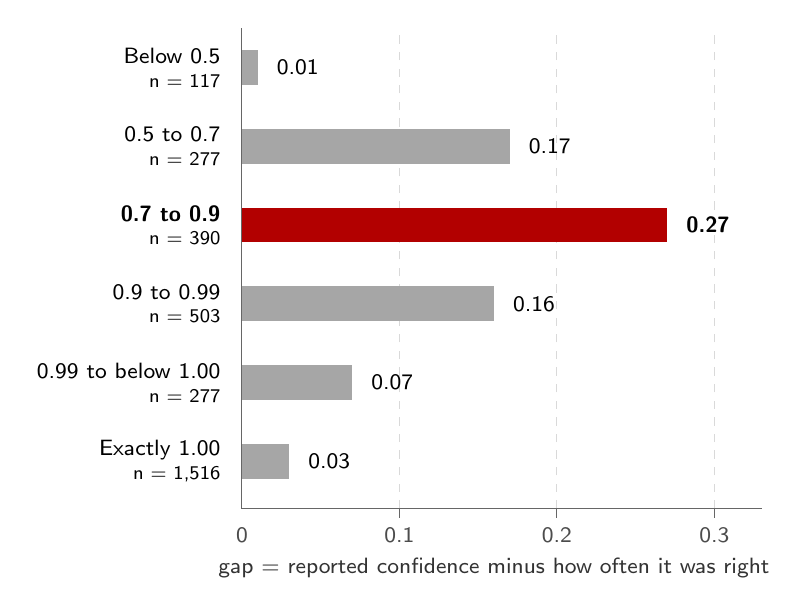
\begin{tikzpicture}[font=\footnotesize\sffamily]
  % light grid and axis
  \foreach \x/\t in {2/0.1, 4/0.2, 6/0.3} {
    \draw[black!15, dashed] (\x,-0.6) -- (\x,5.5);
    \draw[black!60] (\x,-0.6) -- (\x,-0.72);
    \node[anchor=north, text=black!70] at (\x,-0.72) {\t};
  }
  \draw[black!60] (0,-0.6) -- (6.6,-0.6);
  \draw[black!60] (0,-0.6) -- (0,5.5);
  \node[anchor=north, text=black!70] at (0,-0.72) {0};

  % bars, top to bottom
  \fill[black!35] (0,4.78) rectangle (0.2,5.22);
  \node[anchor=east, align=right] at (-0.15,5) {Below 0.5\\[-1pt]{\scriptsize n = 117}};
  \node[anchor=west] at (0.32,5) {0.01};

  \fill[black!35] (0,3.78) rectangle (3.4,4.22);
  \node[anchor=east, align=right] at (-0.15,4) {0.5 to 0.7\\[-1pt]{\scriptsize n = 277}};
  \node[anchor=west] at (3.52,4) {0.17};

  \fill[red!70!black] (0,2.78) rectangle (5.4,3.22);
  \node[anchor=east, align=right] at (-0.15,3) {\textbf{0.7 to 0.9}\\[-1pt]{\scriptsize n = 390}};
  \node[anchor=west] at (5.52,3) {\textbf{0.27}};

  \fill[black!35] (0,1.78) rectangle (3.2,2.22);
  \node[anchor=east, align=right] at (-0.15,2) {0.9 to 0.99\\[-1pt]{\scriptsize n = 503}};
  \node[anchor=west] at (3.32,2) {0.16};

  \fill[black!35] (0,0.78) rectangle (1.4,1.22);
  \node[anchor=east, align=right] at (-0.15,1) {0.99 to below 1.00\\[-1pt]{\scriptsize n = 277}};
  \node[anchor=west] at (1.52,1) {0.07};

  \fill[black!35] (0,-0.22) rectangle (0.6,0.22);
  \node[anchor=east, align=right] at (-0.15,0) {Exactly 1.00\\[-1pt]{\scriptsize n = 1,516}};
  \node[anchor=west] at (0.72,0) {0.03};

  \node[align=center, text=black!80] at (3.2,-1.35) {gap = reported confidence minus how often it was right};
\end{tikzpicture}
\end{document}
